\section{Assignment 6}
\subsection{Feature selection}
We needed to find the quantitative features, which are responsible for the same aspect. We do not have plenty of such features to choose, so we selected features that in our opinion are responsible to the attitude of the readers to the article: \texttt{num\_imgs},\texttt{global\_sentiment\_polarity},  \texttt{shares}. 

\subsection{Visualization with PCA}
To visualize our subsample of the data including three above features and entities, responsible for positive  and negative mood of article context (we exclude neutral mood), we will apply the PCA. But firstly we will standardized data both with ranges and with z-scoring. Scatterplot of standardized subset of data represented at Figure

\begin{figure}[h]
\begin{minipage}[h]{0.49\linewidth}
\center{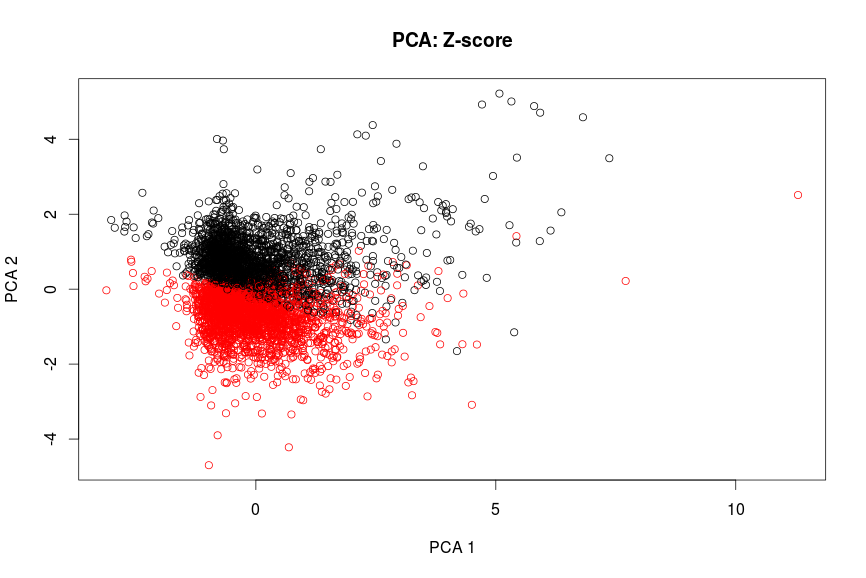
\includegraphics[width=\linewidth]{PCA_zscore_hw6.png} \\ a)}
\end{minipage}
\hfill
\begin{minipage}[h]{0.49\linewidth}
\center{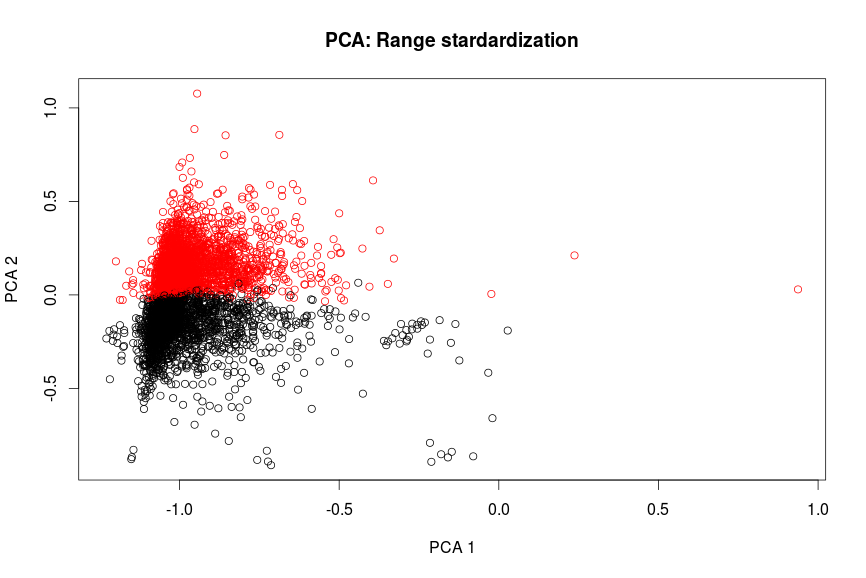
\includegraphics[width=1\linewidth]{PCA_rangenorm_hw6.png} \\ b)}
\end{minipage}
\caption{Scatter plots of 3D-data (\texttt{num\_imgs},\texttt{global\_sentiment\_polarity},  \texttt{shares}) with different standardixation: z-scoring (a) and range standardization (b). Entities, responsible for articles with positive or negative overtones are marked as red and black points respectively.}
\label{fig:PCA_hw6}
\end{figure}

\subsection{Hidden factor}
